\documentclass{article}
\usepackage{amsmath}
\usepackage{graphicx}
\usepackage[margin=1in]{geometry}
\usepackage{hyperref}
\usepackage{caption}
\usepackage{float}
\graphicspath{{images/}}
\hypersetup{
    colorlinks=true,
    urlcolor=blue,
}
\begin{document}

\title{The Dimension of Mutually Recursive Fractals}
\author{Aresh Pourkavoos}
\maketitle

Once upon a time, I was playing with a
\href{https://processing.org}{Processing}
program I had written to draw binary trees.
\begin{figure}[H]
  \centering
  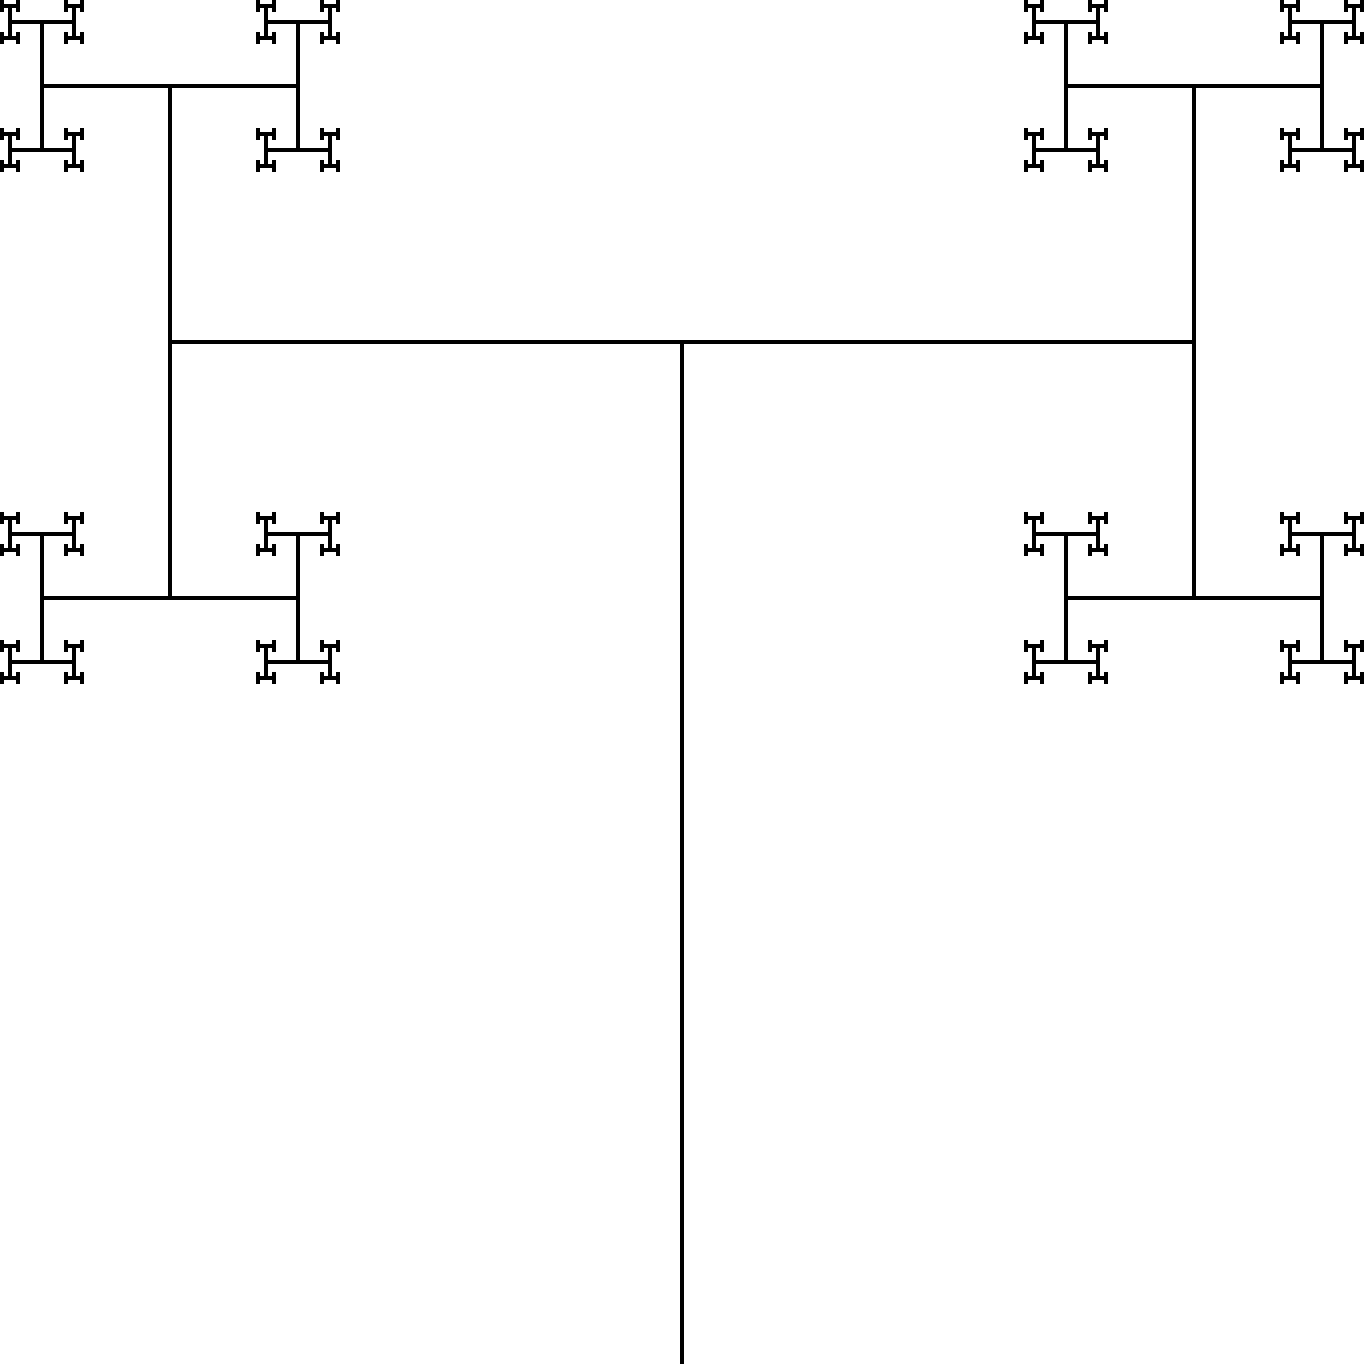
\includegraphics[scale=0.125]{binary_tree.png}
  \caption*{A binary tree drawn by the program.}
\end{figure}
This tree of height $h$ is drawn by drawing
a trunk of height $h$ (a straight line)
and two smaller trees of height $\frac{h}{2}$
coming out at right angles.
However, this tree looks very sparse,
more like a dead tree or one that has lost its leaves for the winter.
In the interest of lushness, I decided to fill in some of the empty space
by adding branches to the trunk:
two of them, coming out at right angles from the center of the trunk
and with height $\frac{h}{4}$ (to be smaller than the main branches).
The program drew the following tree.
\begin{figure}[H]
  \centering
  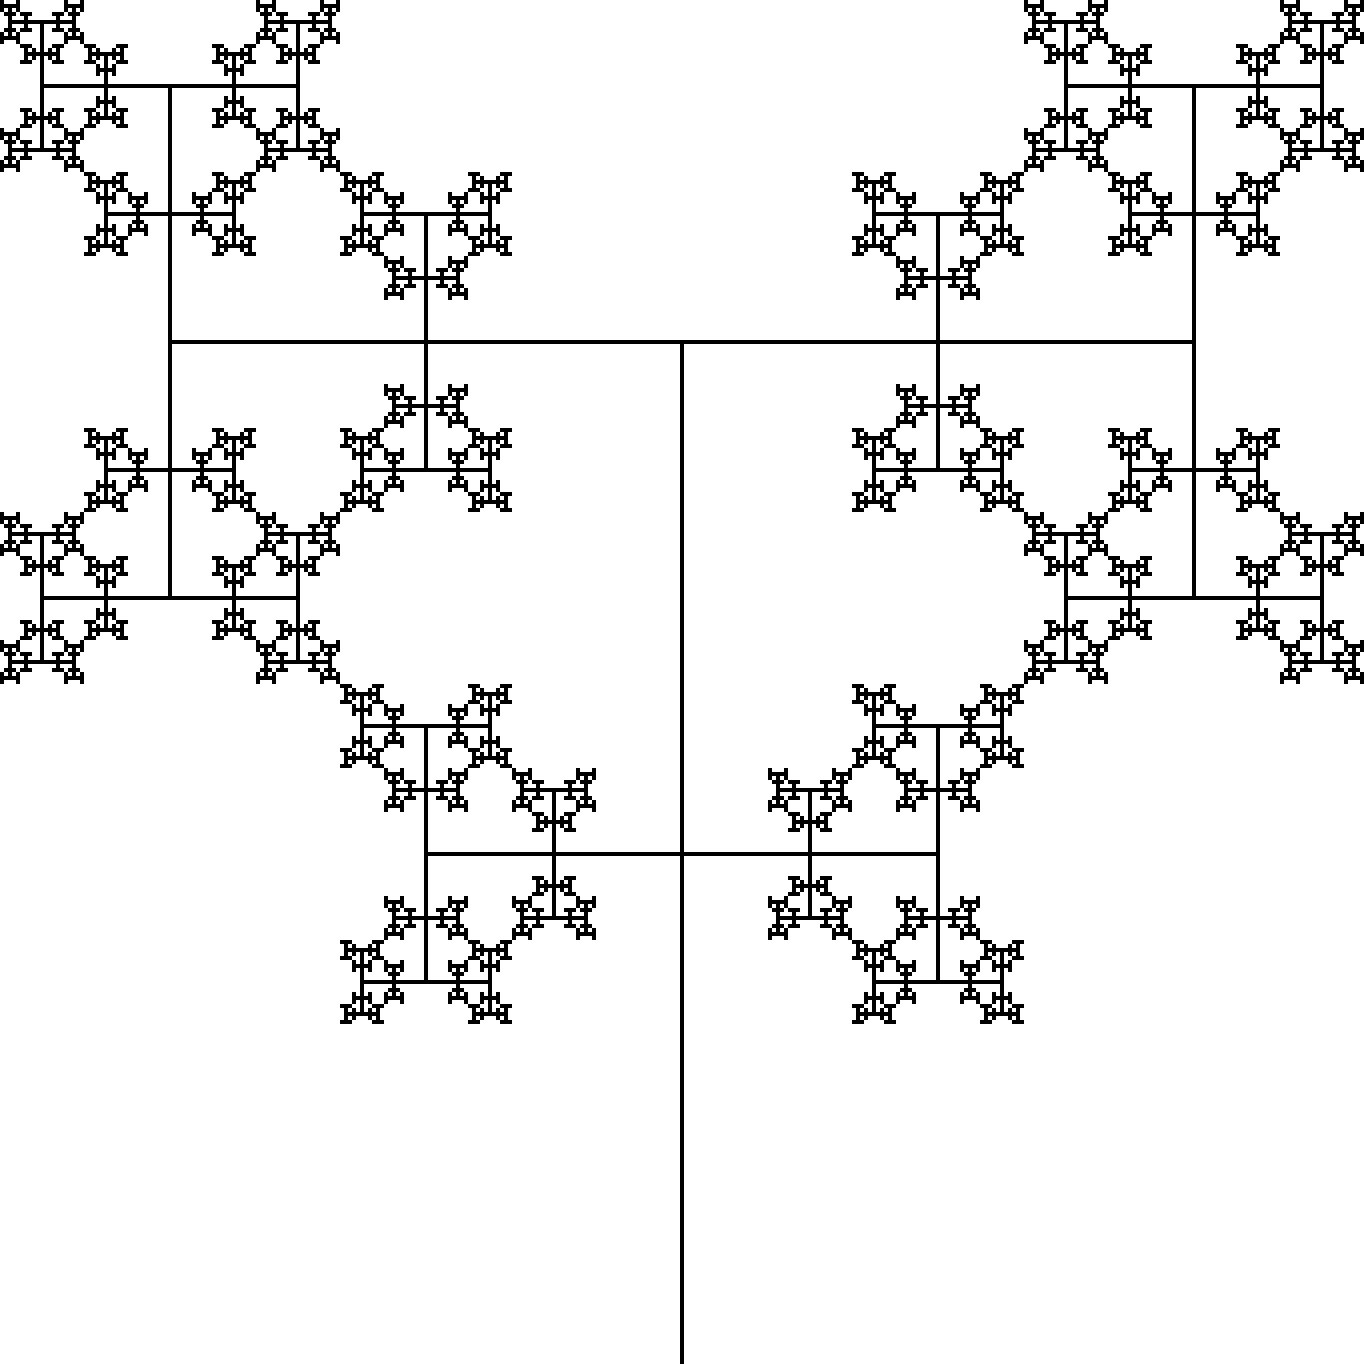
\includegraphics[scale=0.125]{quaternary_tree.png}
\end{figure}
This looks a bit more interesting and a bit less dead.
The tree's ``leaves'' look like they form long chains,
but they're disconnected if you look closely enough.
The large and small branches seem to just barely touch without overlapping.

Most importantly, there was still plenty of empty space
in the form of long segments with no branches.
I wanted to add more branches to the trunk,
but the code was getting longer
and it was becoming tedious to calculate where to place each new branch.
Then, I had the idea of using \textbf{mutual recursion}.

The functions which draw the trees above are recursive in the normal sense,
since each one calls itself to create the smaller branches.
On the other hand,
\textbf{mutually recursive functions call each other.}
I wrote a new function to draw the trunk,
which draws the two smaller trees (branches) as before,
but which also draws \textbf{two trunks} of height $\frac{h}{2}$
stacked on top of each other.
That way, the half-trunks
would themselves draw new, even smaller branches,
as well as even smaller quarter-trunks, etc.
In the limit, each trunk would spawn an infinite number of branches,
each new round smaller than the last,
eventually filling all of the empty space on the trunk of the original tree!

The program spat out this.
\begin{figure}[H]
  \centering
  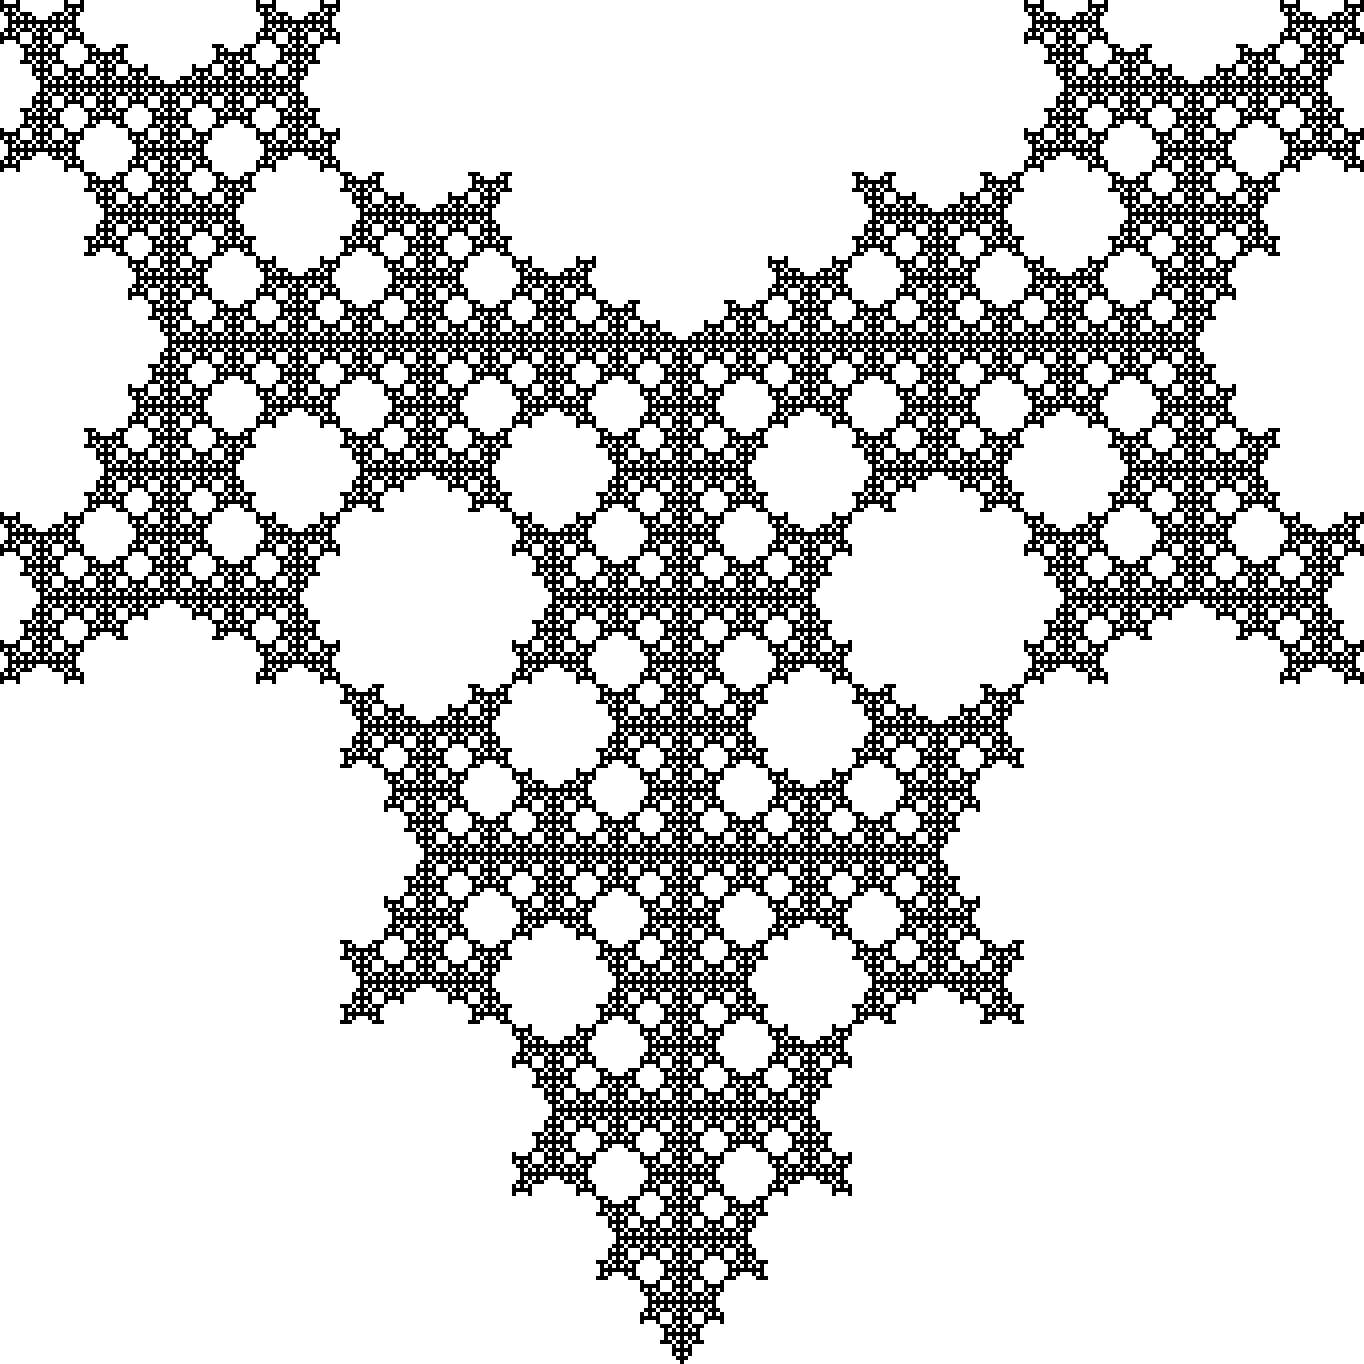
\includegraphics[scale=0.125]{tree.png}
  \caption*{The mutually recursive tree.}
\end{figure}
The new shape jumped out at me.
The tree now has a clearly-defined inside and outside,
there no longer seems to be a distinction between tree and trunk if you zoom in enough,
there are symmetrical shapes in its negative space that remind me of lace doilies,
and the entire thing looks like the skull of a dog or similar animal.
\begin{figure}[H]
  \centering
  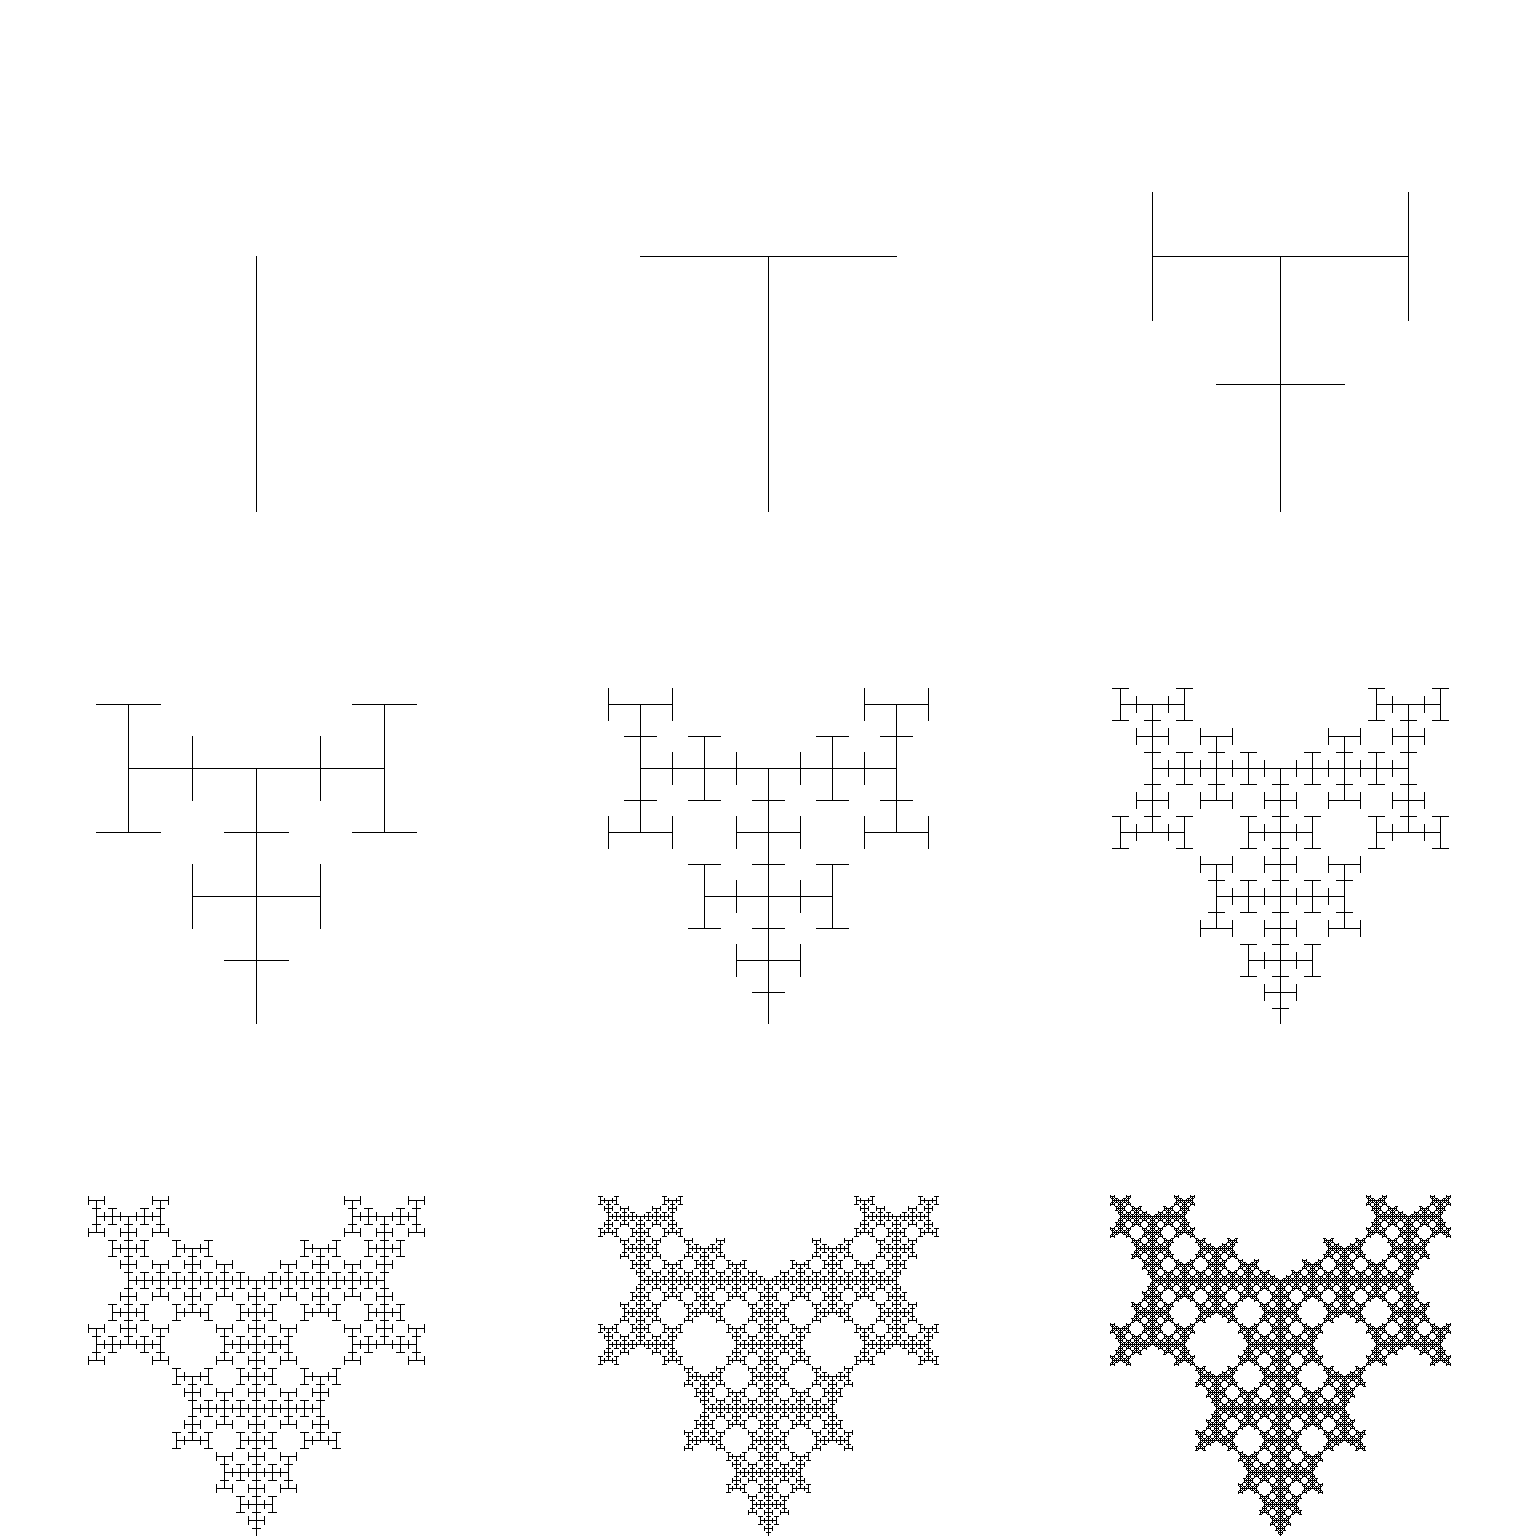
\includegraphics[scale=0.125]{tree_composite.png}
  \caption*{The first few iterations.}
\end{figure}
\begin{figure}[H]
  \centering
  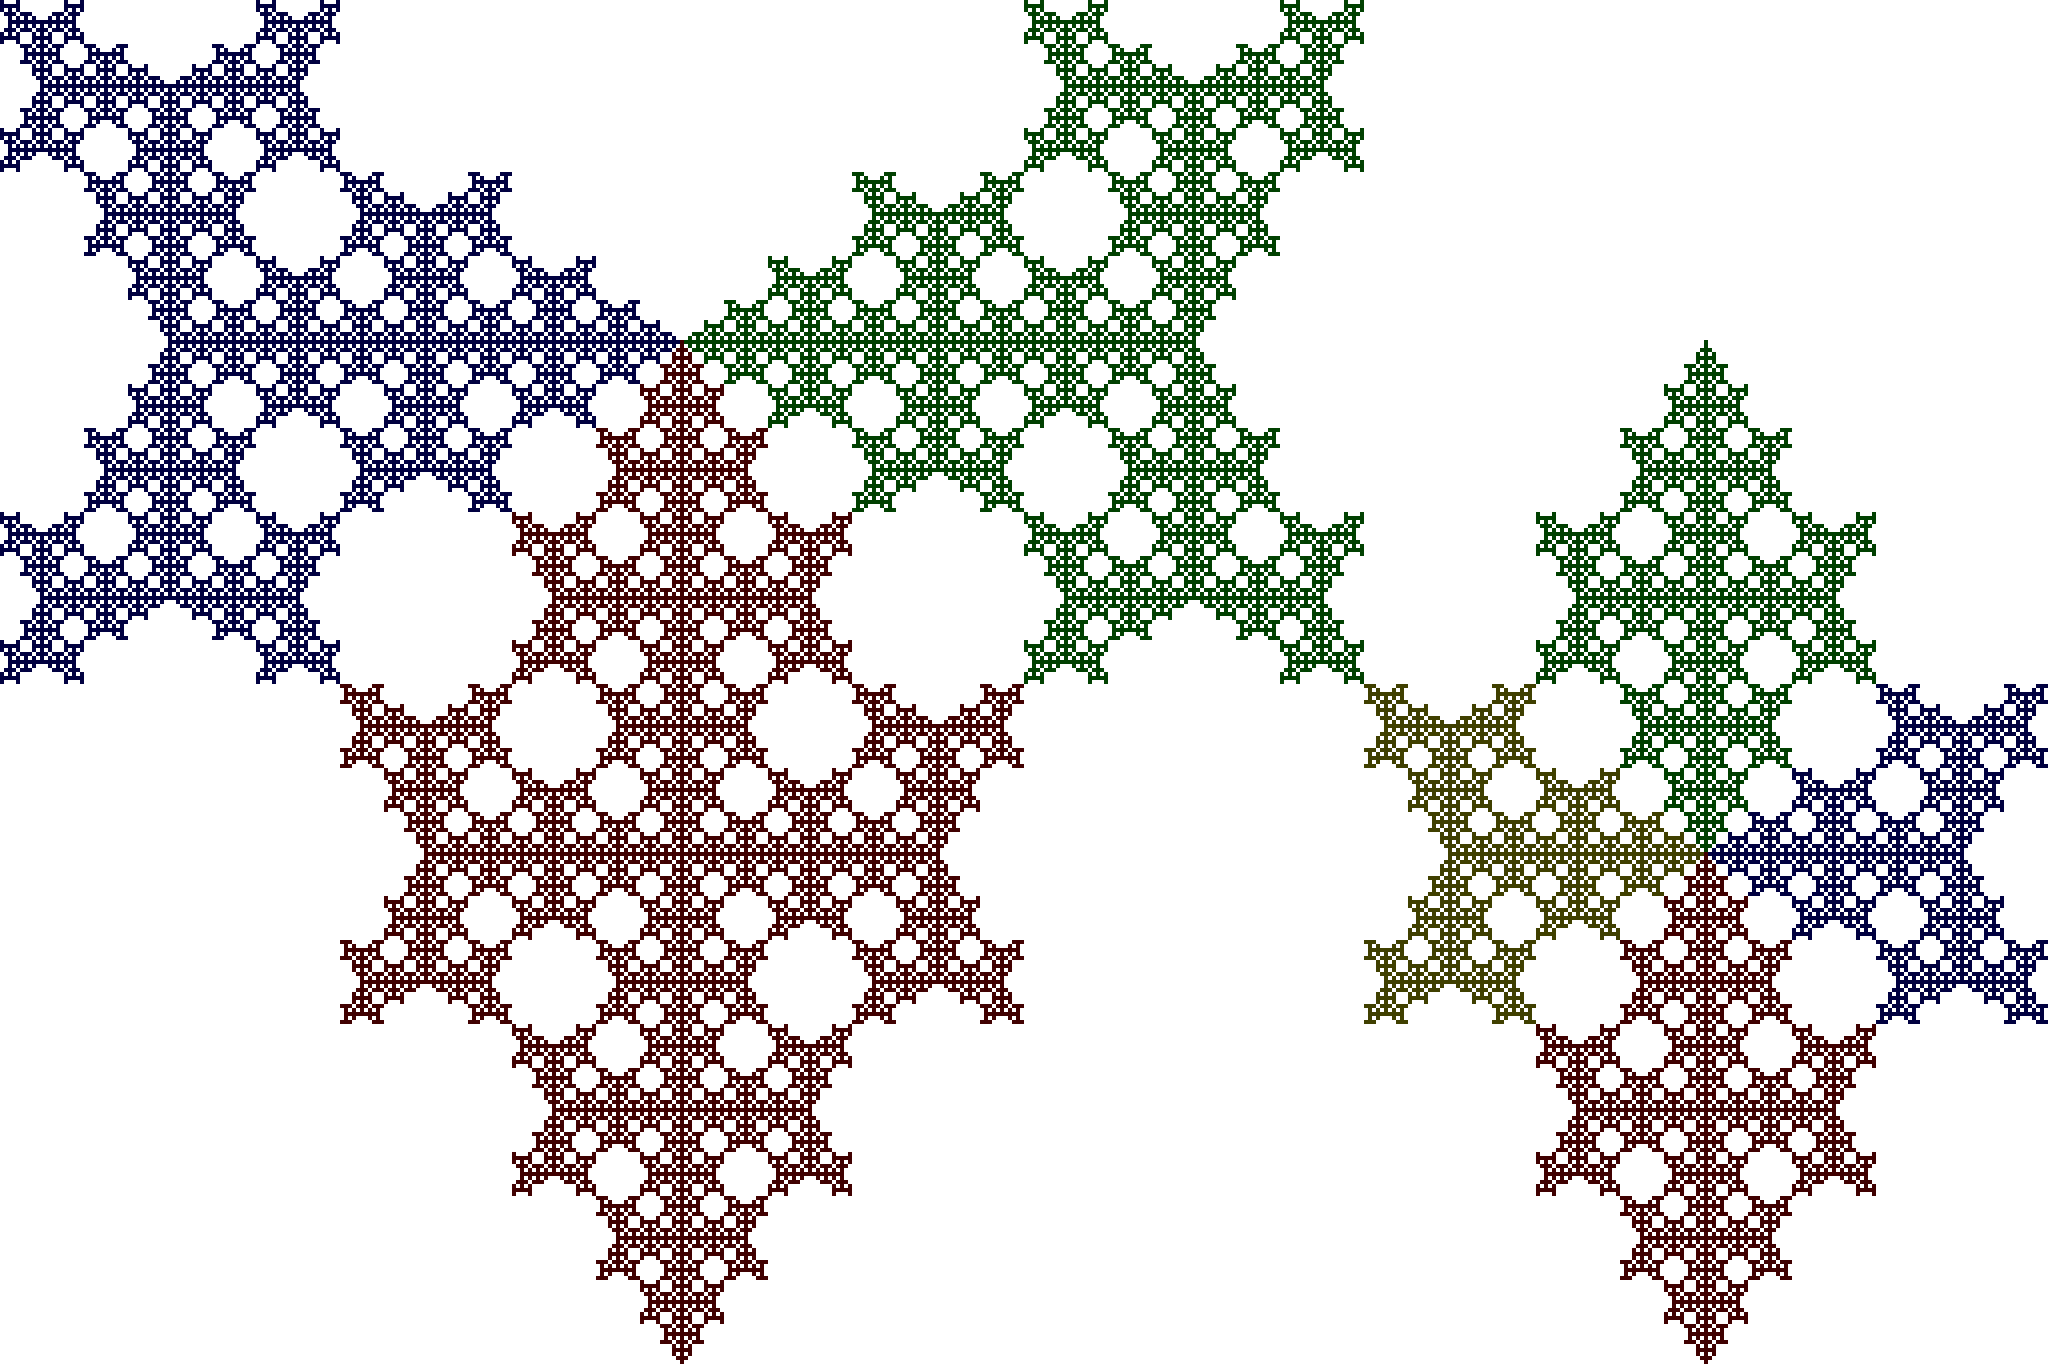
\includegraphics[scale=0.125]{tree_colored.png}
  \caption*{The tree (left) and its trunk (right),
  color-coded to show the elements of each.}
\end{figure}
Needless to say, I was intrigued.
I had never seen this shape before,
and one question that came to mind was
``What is its fractal dimension?''
If you aren't familiar with the idea of fractal dimension,
\href{https://www.youtube.com/watch?v=gB9n2gHsHN4}{this video}
offers a great explanation with nice visuals.
The first nine minutes or so are all you need for the next section
(since this tree is perfectly self-similar),
but I would highly recommend the entire video anyway.

By the (simplified) definition of the fractal dimension $D$,
when we scale the tree by some factor $s$,
its ``mass'' is scaled by the factor $s^D$.
Since the tree is built (at least partially) out of copies half its size,
setting $s=\frac{1}{2}$ seems like a reasonable choice.
Let $f=s^D=\left(\frac{1}{2}\right)^D$ be the mass scaling factor.
We will solve for $f$ first.
Let our original tree have mass $1$,
so its two largest branches, being scaled down by half, have a combined mass of $2f$.
Along with the mass $t$ of the trunk, we can write the mass of the whole tree:
\[1 = 2f+t.\]
But, what exactly is $t$?
First, note that the trunk contains two branches a quarter of the size of the original tree.
Since their mass has been scaled by $f$ twice, their total mass is $2f^2$.
The rest of the trunk, as per its mutually recursive definition,
is made of two half-sized trunks.
As mentioned previously, the trees and trunks look the same when zoomed in on,
so we make the implicit assumption that the trunk has the same fractal dimension as the whole tree.
With this in mind, the two smaller trunks have a combined mass of $2tf$.
Adding this to the quarter-sized branches, we have our second equation:
\[t = 2f^2+2tf.\]
From here, we can solve for $t$ in terms of $f$:
\begin{align*}
  t-2tf &= 2f^2 \\
  t &= \frac{2f^2}{1-2f}
\end{align*}
and substitute into the first equation:
\begin{align*}
  1 &= 2f+\frac{2f^2}{1-2f}\\
  1-2f &= 2f(1-2f)+2f^2\\
  &= 2f-4f^2+2f^2\\
  &= 2f-2f^2 \\
  2f^2-4f+1 &= 0.
\end{align*}
Finally, we can solve for $f$ using the quadratic formula:
\begin{align*}
  f = \frac{4\pm\sqrt{16-8}}{4} = 1\pm\frac{1}{\sqrt{2}}
\end{align*}
Since a half-sized tree has less mass than a full-sized one, $f<1$,
so the solution $f=1-\frac{1}{\sqrt{2}}$ is correct.
Thus, by the definition of $f$,
\begin{align*}
  D &= \log_{\frac{1}{2}}(f)\\
  &= -\log_2(f)\\
  &= \log_2\left(\frac{1}{f}\right)\\
  &= \log_2\left(\frac{1}{1-\frac{1}{\sqrt{2}}}\right)\\
  &= \log_2\left(\frac{1}{\frac{\sqrt{2}-1}{\sqrt{2}}}\right)\\
  &= \log_2\left(\frac{\sqrt{2}}{\sqrt{2}-1}\right)\\
  &= \log_2\left(\frac{\sqrt{2}(\sqrt{2}+1)}{(\sqrt{2}-1)(\sqrt{2}+1)}\right)\\
  &= \log_2\left(\frac{2+\sqrt{2}}{\sqrt{2}^2-1^2}\right)\\
  &= \log_2\left(2+\sqrt{2}\right)\\
  &\approx 1.7716
\end{align*}
%% \begin{figure}[H]
%%   \centering
%%   \includegraphics{sierpinski.png}
%%   \caption*{The Sierpinski triangle, }
%% \end{figure}

%% First, rewrite the tree and trunk of height $h$
%% in terms of trees and trunks of height $h/2$.
%% Within the trunk of height $h$,
%% 1 of the trunks of height $h/2$
%% and the 2 trees of height $h/4$
%% make up a tree of height $h/2$.
%% Thus a trunk of height $h$ is
%% 1 trunk of height $h/2$
%% and 1 tree of height $h/2$.
%% Within the tree of height $h$,
%% the trunk of height $h$
%% can be rewritten with this new definition.
%% Thus a tree of height $h$ is
%% 1 trunk of height $h/2$
%% and 3 trees of height $h/2$.

%% Let $a$ be
%% the ``mass'' (measure?) of a trunk with height $h/2$,
%% and let $b$ be
%% the mass of a tree with height $h/2$.
%% Then the mass of a trunk with height $h$ is $a+b$,
%% and the mass of a tree with height $h$ is $a+3b$.
%% Thus the (linear) transformation which maps
%% the vector $\begin{bmatrix} a\\b \end{bmatrix}$
%% to the vector $\begin{bmatrix} a+b\\a+3b \end{bmatrix}$
%% scales the heights of a trunk and a tree by $2$.
%% It can be represented by
%% the matrix $\begin{bmatrix} 1&1\\1&3 \end{bmatrix}$.
%% Assume that trunks and trees have the same Hausdorff dimension $d$.
%% (Proving this may be nontrivial, but
%% the interiors of trees and trunks are visually similar.)
%% Thus scaling a tree's (or a trunk's) height by a factor of $2$
%% scales its mass by a factor of $2^d$.
%% Call this quantity $\lambda$.
%% Since the matrix $\begin{bmatrix} 1&1\\1&3 \end{bmatrix}$

%% Use the writeidea command to edit.

\end{document}
